\documentclass[12pt,letterpaper]{article}

\usepackage[utf8]{inputenc}
\usepackage[T1]{fontenc}
\usepackage[english]{babel}
\usepackage{amsmath, amssymb, amsthm}
\usepackage{float, enumitem, xcolor, geometry}
\usepackage{graphicx, fancyhdr, fancyvrb}
\usepackage{array, makecell}
\usepackage{forest}
\usepackage[normalem]{ulem}
\usepackage[colorlinks=true, linkcolor=linkblue, urlcolor=linkblue, citecolor=linkblue]{hyperref}
\usepackage{makecell}
\usepackage{tikz}
\usepackage{svg}
\usetikzlibrary{automata, positioning, arrows.meta}

\definecolor{linkblue}{HTML}{1A167A}

\geometry{margin=2cm, top=2cm, bottom=2cm}

\newcommand{\pred}{$\rightarrow$}
\newcommand{\asig}{$\leftarrow$}

\newcommand{\nt}[1]{\textit{#1}}
\newcommand{\tk}[1]{\texttt{#1}}
\newcommand{\tx}[1]{\text{#1}}
\newcommand{\First}[1]{\mathrm{FIRST}(#1)}
\newcommand{\Follow}[1]{\mathrm{FOLLOW}(#1)}
\newcommand{\eps}{\varepsilon}

% ========================================
% COLORES
% ========================================
\definecolor{green_checkmark}{HTML}{07E314}
\definecolor{red_cross}{HTML}{ED4728}

% ========================================
% COMANDOS PARA MARCADORES
% ========================================
\newcommand{\greencheck}{\textcolor{green_checkmark}{$\checkmark$}}
\newcommand{\redcross}{\textcolor{red_cross}{$\times$}}

% ========================================
% CONSTANTES DEL ENCABEZADO
% ========================================
\newcommand{\encabezadoIzq}{Compiladores 2027-1}
\newcommand{\encabezadoCen}{Tarea 2}
\newcommand{\encabezadoDer}{\textit{Minim, deriv, elim y EBNF}}

% ========================================
% CONFIGURACION DEL ENCABEZADO
% ========================================
\pagestyle{fancy}
\fancyhf{}

\fancyhead[L]{\encabezadoIzq}
\fancyhead[C]{\encabezadoCen}
\fancyhead[R]{\encabezadoDer}

\fancyfoot[C]{\thepage}

\renewcommand{\headrulewidth}{0.1pt}
\renewcommand{\footrulewidth}{0pt}

% ========================================
% CONFIGURACION DE TABLAS
% ========================================
\newcolumntype{C}[1]{>{\centering\arraybackslash}m{#1}}
\newcolumntype{L}[1]{>{\raggedright\arraybackslash}m{#1}}
\newcolumntype{R}[1]{>{\raggedleft\arraybackslash}m{#1}}

\begin{document}

\thispagestyle{empty}
\begin{titlepage}
  \thispagestyle{empty}
  %--------------- COMANDO LINEA----------------->
  \newcommand{\linea}{\rule{\linewidth}{0.5mm}}                 
  \center
  %<<<<<<<<<<<<<<<<<<<<<<<<<<<<<<<<<<<<<<<<<<<

  %Add logos
  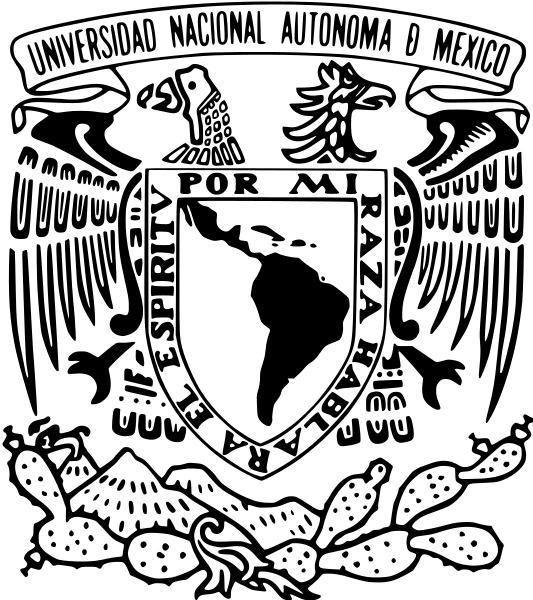
\includegraphics[width=0.24\textwidth]{../unam_logo.png} \hspace{1.5cm}
  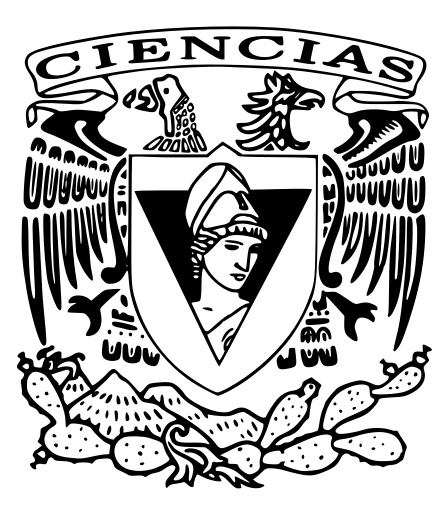
\includegraphics[width=0.25\textwidth]{../fc_logo.png} \\[1cm]
  \textbf{\Large UNIVERSIDAD NACIONAL AUTÓNOMA}\\[3mm]
  \textbf{\Large DE MÉXICO} \\[6mm]
  \textit{\Large Facultad de Ciencias}

  \vfill

  %---------------TÍTULO----------------->
  \linea
  \vfill \vspace{1cm}
  \textbf{\Large Compiladores}\\[1.1cm]
  \textbf{\Large Conjunto \textsc{First} y  \textsc{Follow}}\\[0.9cm]
  \linea \\
  \vfill
  \vspace{0.7cm}
  %Title of the Research
  \textbf{\Large  Tarea 4}\\[6mm]
  %<<<<<<<<<<<<<<<<<<<<<<<<<<<<<<<<<<<<<<<<<<<

  %Team
  \vfill
  \textit{\small Presenta:}\\
  \textbf{\large  \textbf{Ramírez Juárez María Fernanda} - 321204747}\\[3mm]
  \textbf{\large  \textbf{Rojo Peña Manuel Ianluck} - 118005762}\\[3mm]

  %Profesor y Grupo
  \textit{\small Profesor:}\\
  \textbf{Pablo Martínez Yessica Janeth}\\[3mm]
  \textit{\small Ayudante:}\\
  \textbf{Rojas Fuentes Andrea}\\[3mm]
  \small Grupo: 7010, 2027-1\\[3mm]
  \vfill

  %Fecha or Date
  \textit{\small Fecha de entrega:}\\
         {\large 7 de octubre, 2026}
         
\end{titlepage}


%%%%%%%%%%%%%%%%%%%%%%%%%%%%%%%%%%%%%%%%%%
\newpage
%%%%%%%%%%%%%%%%%%%%%%%%%%%%%%%%%%%%%%%%%%

\begin{enumerate}[label=\arabic*.]

\item Obtenga el conjunto \textsc{First} y \textsc{Follow} de cada una de las siguientes gramáticas mostrando el
  procedimiento completo así como se vió en clase. Además construya la tabla final de análisis sintáctico
  \nt{LL(1)} y muestre su proceso detalladamente para obtenerla así como se vió en clase:
  
  \begin{itemize}
  \item Gramática 1:
    \[
    \begin{aligned}
      \nt{A} &\to \tx{B}\ \tx{C}\ \tx{D}\\
      \nt{B} &\to \bf{a}\ \tx{C}\ \bf{b} \mid \eps \\
      \nt{C} &\to \bf{c}\ \tx{A}\ \bf{d} \mid \bf{e}\ \tx{B}\ \bf{f} \mid \bf{g}\ \tx{D}\ \bf{h} \mid \eps \\
      \nt{D} &\to \bf{i}
    \end{aligned}
    \]

    \bigskip
    
    \textbf{Paso 1. Anulables}\\
    Solo \nt{B} y \nt{C} tienen la producción $\eps$. \nt{D} siempre produce \tk{i} y \nt{A} empieza con \nt{B}\,
    \nt{C}\,\nt{D}, que incluye a \nt{D}, así que \nt{A} tampoco es anulable.\\

    \textbf{Paso 2. \textsc{First}}\\
    Partimos de lo que no depende de nadie:
    \[
    \begin{aligned}
      \First{\tx{D}} &= \{\tk{i}\} \\
      \First{\tx{B}} &= \{\tk{a}\} \cup \{\eps\} = \{\tk{a},\ \eps\} \\
      \First{\tx{C}} &= \{\tk{c}\} \cup \{\tk{e}\} \cup \{\tk{g}\} \cup \{\eps\} = \{\tk{c},\ \tk{e},\ \tk{g},\
      \eps\}
    \end{aligned}
    \]
    
    Para \nt{A} recorremos $\nt{B}\,\nt{C}\,\nt{D}$ de izquierda a derecha, avanzando mientras el símbolo sea
    anulable:
    \[
    \begin{aligned}
      \First{\tx{A}} &= \big(\ \First{\tx{B}}\setminus\{\eps\}\ \big)
                        \cup
                        \big(\ \First{\tx{C}}\setminus\{\eps\}\ \big)
                        \cup
                        \First{\tx{D}} \\
                     &= \{\tk{a}\} \cup \{\tk{c},\tk{e},\tk{g}\} \cup \{\tk{i}\} \\
                     &= \{\tk{a},\ \tk{c},\ \tk{e},\ \tk{g},\ \tk{i}\}
    \end{aligned}
    \]
    El recorrido se detiene en \nt{D} porque no es anulable, así que $\eps \notin \First{\nt{A}}$. \footnote{Restamos $\eps$ de $\First{\tx{B}}$ y $\First{\tx{C}}$ porque $\eps$ no es un símbolo de la entrada, solo indica que
    ese símbolo puede desaparecer y que el recorrido debe continuar con el siguiente. Incluiríamos $\eps$ en
    $\First{\tx{A}}$ únicamente si $\nt{B}$, $\nt{C}$ y $\nt{D}$ fueran todos anulables.} \\
    
    Por lo tanto, el conjunto \textsc{First} de la gramática es:
    \[
    \begin{aligned}
      \First{\tx{A}} &= \{\tk{a},\ \tk{c},\ \tk{e},\ \tk{g},\ \tk{i}\} \\
      \First{\tx{B}} &= \{\tk{a},\ \eps\} \\
      \First{\tx{C}} &= \{\tk{c},\ \tk{e},\ \tk{g},\ \eps\}\\
      \First{\tx{D}} &= \{\tk{i}\}
    \end{aligned}
    \]

    \newpage
    
    \textbf{Paso 3. \textsc{Follow}}\\
    \begin{itemize}
    \item $\Follow{\tx{A}}$: \nt{A} es el símbolo inicial, así que aporta \tk{\$}.
      En $\nt{C}\to\tk{c}\,\nt{A}\,\tk{d}$ le sigue \tk{d}.
      \[
      \Follow{\nt{A}} = \{\tk{\$},\ \tk{d}\}
      \]
      
    \item $\Follow{\tx{B}}$: en $\nt{A}\to\nt{B}\,\nt{C}\,\nt{D}$ le sigue $\nt{C}\,\nt{D}$.\\
      $\First{\nt{C}\,\nt{D}} = \{\tk{c},\tk{e},\tk{g}\}\cup\{\tk{i}\}$, porque \nt{C} es anulable y entonces se
      agrega $\First{\nt{D}}$.\\
      En $\nt{C}\to\tk{e}\,\nt{B}\,\tk{f}$ le sigue \tk{f}.
      \[
      \Follow{\nt{B}} = \{\tk{c},\ \tk{e},\ \tk{g},\ \tk{i},\ \tk{f}\}
      \]
      
    \item $\Follow{\nt{C}}$: en $\nt{A}\to\nt{B}\,\nt{C}\,\nt{D}$ le sigue \nt{D}, así que se agrega $\First{\nt{D}}=\{\tk{i}\}$.\\
      En $\nt{B}\to\tk{a}\,\nt{C}\,\tk{b}$ le sigue \tk{b}.\\
      \nt{C} nunca queda al final de una producción, así que no se hereda ningún \textsc{Follow}.
      \[
      \Follow{\nt{C}} = \{\tk{i},\ \tk{b}\}
      \]
      
    \item $\Follow{\nt{D}}$: en $\nt{A}\to\nt{B}\,\nt{C}\,\nt{D}$ está al final, así que hereda
      $\Follow{\nt{A}}$.\\
      En $\nt{C}\to\tk{g}\,\nt{D}\,\tk{h}$ le sigue \tk{h}.
      \[
      \Follow{\nt{D}} = \{\tk{\$},\ \tk{d},\ \tk{h}\}
      \]
    \end{itemize}

    Al repetir las reglas ningún conjunto vuelve a cambiar, por lo que ya es el punto fijo.\\

    Por lo tanto, el conjunto \textsc{Follow} de la gramática es:
    \[
    \begin{aligned}
      \Follow{\tx{A}} &= \{\tk{\$},\ \tk{d}\} \\
      \Follow{\tx{B}} &= \{\tk{c},\ \tk{e},\ \tk{g},\ \tk{i},\ \tk{f}\} \\
      \Follow{\tx{C}} &= \{\tk{i},\ \tk{b}\} \\
      \Follow{\tx{D}} &= \{\tk{\$},\ \tk{d},\ \tk{h}\}
    \end{aligned}
    \]
    
    \textbf{Paso 4. Producciones enumeradas y su selección}
    \[
    \begin{array}{c l l l}
      \# & \text{Producción} & \text{Colocado en} & \text{Motivo} \\ \hline
      1 & \nt{A}\to\nt{B}\,\nt{C}\,\nt{D} & \tk{a},\tk{c},\tk{e},\tk{g},\tk{i} & \First{\nt{B}\,\nt{C}\,\nt{D}} \\
      2 & \nt{B}\to\tk{a}\,\nt{C}\,\tk{b} & \tk{a} & \text{\textsc{First}} \\
      3 & \nt{B}\to\eps & \tk{c},\tk{e},\tk{g},\tk{i},\tk{f} & \Follow{\nt{B}} \\
      4 & \nt{C}\to\tk{c}\,\nt{A}\,\tk{d} & \tk{c} & \text{\textsc{First}} \\
      5 & \nt{C}\to\tk{e}\,\nt{B}\,\tk{f} & \tk{e} & \text{\textsc{First}} \\
      6 & \nt{C}\to\tk{g}\,\nt{D}\,\tk{h} & \tk{g} & \text{\textsc{First}} \\
      7 & \nt{C}\to\eps & \tk{i},\tk{b} & \Follow{\nt{C}} \\
      8 & \nt{D}\to\tk{i} & \tk{i} & \text{\textsc{First}}
    \end{array}
    \]

    \newpage
    
    \textbf{Paso 5. Tabla LL(1)}
    \[
    \begin{array}{c|c|c|c|c|c|c|c|c|c|c}
      & \tk{a} & \tk{b} & \tk{c} & \tk{d} & \tk{e} & \tk{f} & \tk{g} & \tk{h} & \tk{i} & \tk{\$} \\ \hline
      \nt{A} & 1 &   & 1 &   & 1 &   & 1 &   & 1 &   \\ \hline
      \nt{B} & 2 &   & 3 &   & 3 & 3 & 3 &   & 3 &   \\ \hline
      \nt{C} &   & 7 & 4 &   & 5 &   & 6 &   & 7 &   \\ \hline
      \nt{D} &   &   &   &   &   &   &   &   & 8 &   \\
    \end{array}
    \]

    Ninguna celda tiene más de una producción, en particular, para \nt{B}:\\
    $\First{\tk{a}\,\nt{C}\,\tk{b}}=\{\tk{a}\}$ y $\Follow{\nt{B}}=\{\tk{c},\tk{e},\tk{g},\tk{i},\tk{f}\}$
    son disjuntos.\\
    Para \nt{C}:
    $\{\tk{c},\tk{e},\tk{g}\}\cap\Follow{\nt{C}}=\{\tk{c},\tk{e},\tk{g}\}\cap\{\tk{i},\tk{b}\}=\varnothing$.\\
    
    \textbf{La Gramática 1 es LL(1).}

    
    %%%%%%%%%%%%%%%%%%%%%%%%%%
    \bigskip
    %%%%%%%%%%%%%%%%%%%%%%%%%%

    
  \item Gramática 2:
    \[
    \begin{aligned}
      \nt{Exp}    &\to \tx{Term}\ \tx{Exp'} \\
      \nt{Exp'}   &\to \tx{Opsuma}\ \tx{Term}\ \tx{Exp'} \mid \\
      \nt{Opsuma} &\to \tk{+} \mid \tk{-} \\
      \nt{Term}   &\to \tx{Factor}\ \tx{Term'} \\
      \nt{Term'}  &\to \tx{Opmult}\ \tx{Factor}\ \tx{Term'} \mid \\
      \nt{Opmult} &\to \tk{*} \\
      \nt{Factor} &\to \textbf{(}\ \tx{Exp}\ \textbf{)} \mid \bf{num}
    \end{aligned}
    \]

    \bigskip

    Tenemos que añadir $\nt{Exp'}\to\eps$ y $\nt{Term'}\to\eps$, pues sin ellas la gramática no deriva ninguna
    cadena, la explicación a este ajuste está más detallada al final del resultado:
    \[
    \begin{aligned}
      \nt{Exp}    &\to \nt{Term}\ \nt{Exp'} \\
      \nt{Exp'}   &\to \nt{Opsuma}\ \nt{Term}\ \nt{Exp'} \mid \eps \\
      \nt{Opsuma} &\to \tk{+} \mid \tk{-} \\
      \nt{Term}   &\to \nt{Factor}\ \nt{Term'} \\
      \nt{Term'}  &\to \nt{Opmult}\ \nt{Factor}\ \nt{Term'} \mid \eps \\
      \nt{Opmult} &\to \tk{*} \\
      \nt{Factor} &\to \tk{(}\ \nt{Exp}\ \tk{)} \mid \tk{num}
    \end{aligned}
    \]

    \bigskip
    
    \textbf{Paso 1. Anulables}\\
    Solo \tx{Exp'} y \tx{Term'} lo son.\\

    \textbf{Paso 2. \textsc{First}}\\
    Primero los que empiezan con terminales:
    \[
    \begin{aligned}
      \First{\tx{Opsuma}} &= \{\tk{+},\ \tk{-}\} \\
      \First{\tx{Opmult}} &= \{\tk{*}\} \\
      \First{\tx{Factor}} &= \{\tk{(},\ \tk{num}\} \\
      \First{\tx{Exp'}}   &= \First{\tx{Opsuma}} \cup \{\eps\} = \{\tk{+},\ \tk{-},\ \eps\} \\
      \First{\tx{Term'}}  &= \First{\tx{Opmult}} \cup \{\eps\} = \{\tk{*},\ \eps\}
    \end{aligned}
    \]
    Después los que dependen de otros. \nt{Factor} no es anulable, así que el cálculo se detiene en él:
    \[
    \First{\nt{Term}} = \First{\nt{Factor}} = \{\tk{(},\ \tk{num}\}, \qquad
    \First{\nt{Exp}} = \First{\nt{Term}} = \{\tk{(},\ \tk{num}\}
    \]

    Por lo tanto, el conjunto \textsc{First} de la gramática es:
    \[
    \begin{aligned}
      \First{\tx{Exp}}    &= \{\tk{(},\ \tk{num}\} \\
      \First{\tx{Exp'}}   &= \{\tk{+},\ \tk{-},\ \eps\} \\
      \First{\tx{Opsuma}} &= \{\tk{+},\ \tk{-}\} \\
      \First{\tx{Term}}   &= \{\tk{(},\ \tk{num}\} \\
      \First{\tx{Term'}}  &= \{\tk{*},\ \eps\} \\
      \First{\tx{Opmult}} &= \{\tk{*}\} \\
      \First{\tx{Factor}} &= \{\tk{(},\ \tk{num}\}
    \end{aligned}
    \]
    
    \textbf{Paso 3. \textsc{Follow}}
    \begin{itemize}
    \item $\Follow{\tx{Exp}}$: es el inicial, así que aporta \tk{\$}.\\
      En $\nt{Factor}\to\tk{(}\,\nt{Exp}\,\tk{)}$ le sigue \tk{)}.
      \[
      \Follow{\tx{Exp}} = \{\tk{\$},\ \tk{)}\}
      \]
      
    \item $\Follow{\tx{Exp'}}$: en $\nt{Exp}\to\nt{Term}\,\nt{Exp'}$ y en
      $\nt{Exp'}\to\nt{Opsuma}\,\nt{Term}\,\nt{Exp'}$ está al final, así que hereda
      $\Follow{\nt{Exp}}$ \big(y $\Follow{\nt{Exp'}}$, que es ella misma\big).
      \[
      \Follow{\tx{Exp'}} = \{\tk{\$},\ \tk{)}\}
      \]
      
    \item $\Follow{\tx{Term}}$: en ambas producciones donde aparece le sigue \nt{Exp'}.\\
      Se agrega $\First{\tx{Exp'}}\setminus\{\eps\}=\{\tk{+},\tk{-}\}$ y, como \nt{Exp'} es anulable, también
      $\Follow{\nt{Exp}}$ \big(y $\Follow{\nt{Exp'}}$ en la segunda producción, que es lo mismo\big).
      \[
      \Follow{\tx{Term}} = \{\tk{+},\ \tk{-},\ \tk{\$},\ \tk{)}\}
      \]
      
    \item $\Follow{\tx{Opsuma}}$: le sigue \nt{Term}, y \nt{Term} no es anulable.
      \[
      \Follow{\tx{Opsuma}} = \First{\tx{Term}} = \{\tk{(},\ \tk{num}\}
      \]
      
    \item $\Follow{\tx{Term'}}$: está al final de $\nt{Term}\to\nt{Factor}\,\nt{Term'}$\\
      y de $\nt{Term'}\to\nt{Opmult}\,\nt{Factor}\,\nt{Term'}$, así que hereda $\Follow{\tx{Term}}$.
      \[
      \Follow{\tx{Term'}} = \{\tk{+},\ \tk{-},\ \tk{\$},\ \tk{)}\}
      \]
      
    \item $\Follow{\tx{Factor}}$: le sigue \nt{Term'}. Se agrega $\First{\tx{Term'}}\setminus\{\eps\}=\{\tk{*}\}$ y, como \nt{Term'} es anulable, también $\Follow{\tx{Term}}$.
      \[
      \Follow{\tx{Factor}} = \{\tk{*},\ \tk{+},\ \tk{-},\ \tk{\$},\ \tk{)}\}
      \]
      
    \item $\Follow{\tx{Opmult}}$: le sigue \nt{Factor}, que no es anulable.
      \[
      \Follow{\tx{Opmult}} = \{\tk{(},\ \tk{num}\}
      \]
    \end{itemize}

    Por lo tanto, el conjunto \textsc{Follow} de la gramática es:
    \[
    \begin{aligned}
      \Follow{\tx{Exp}}    &= \{\tk{\$},\ \tk{)}\} \\
      \Follow{\tx{Exp'}}   &= \{\tk{\$},\ \tk{)}\} \\
      \Follow{\tx{Opsuma}} &= \{\tk{(},\ \tk{num}\} \\
      \Follow{\tx{Term}}   &= \{\tk{+},\ \tk{-},\ \tk{\$},\ \tk{)}\} \\
      \Follow{\tx{Term'}}  &= \{\tk{+},\ \tk{-},\ \tk{\$},\ \tk{)}\} \\
      \Follow{\tx{Opmult}} &= \{\tk{(},\ \tk{num}\} \\
      \Follow{\tx{Factor}} &= \{\tk{*},\ \tk{+},\ \tk{-},\ \tk{\$},\ \tk{)}\}
    \end{aligned}
    \]

    \bigskip
    
    \textbf{Paso 4. Producciones numeradas y su selección}
    \[
    \begin{array}{c l l l}
      \# & \text{Producción} & \text{Colocado en} & \text{Motivo} \\ \hline
      1  & \nt{Exp}\to\nt{Term}\,\nt{Exp'} & \tk{(},\tk{num} & \text{\textsc{First}} \\
      2  & \nt{Exp'}\to\nt{Opsuma}\,\nt{Term}\,\nt{Exp'} & \tk{+},\tk{-} & \text{\textsc{First}} \\
      3  & \nt{Exp'}\to\eps & \tk{\$},\tk{)} & \Follow{\tx{Exp'}} \\
      4  & \nt{Opsuma}\to\tk{+} & \tk{+} & \text{\textsc{First}} \\
      5  & \nt{Opsuma}\to\tk{-} & \tk{-} & \text{\textsc{First}} \\
      6  & \nt{Term}\to\nt{Factor}\,\nt{Term'} & \tk{(},\tk{num} & \text{\textsc{First}} \\
      7  & \nt{Term'}\to\nt{Opmult}\,\nt{Factor}\,\nt{Term'} & \tk{*} & \text{\textsc{First}} \\
      8  & \nt{Term'}\to\eps & \tk{+},\tk{-},\tk{)},\tk{\$} & \Follow{\tx{Term'}} \\
      9  & \nt{Opmult}\to\tk{*} & \tk{*} & \text{\textsc{First}} \\
      10 & \nt{Factor}\to\tk{(}\,\nt{Exp}\,\tk{)} & \tk{(} & \text{\textsc{First}} \\
      11 & \nt{Factor}\to\tk{num} & \tk{num} & \text{\textsc{First}}
    \end{array}
    \]

    \bigskip
    
    \textbf{Paso 5. Tabla LL(1)}
    \[
    \begin{array}{c|c|c|c|c|c|c|c}
      & \tk{+} & \tk{-} & \tk{*} & \tk{(} & \tk{)} & \tk{num} & \tk{\$} \\ \hline
      \nt{Exp}     &   &   &   & 1  &   & 1  &   \\ \hline
      \nt{Exp'}    & 2 & 2 &   &    & 3 &    & 3 \\ \hline
      \nt{Opsuma}  & 4 & 5 &   &    &   &    &   \\ \hline
      \nt{Term}    &   &   &   & 6  &   & 6  &   \\ \hline
      \nt{Term'}   & 8 & 8 & 7 &    & 8 &    & 8 \\ \hline
      \nt{Opmult}  &   &   & 9 &    &   &    &   \\ \hline
      \nt{Factor}  &   &   &   & 10 &   & 11 &   \\
    \end{array}
    \]

    Ninguna celda tiene dos producciones.\\
    Para \nt{Exp'}:
    $\First{\tx{Opsuma}\ldots}=\{\tk{+},\tk{-}\}$ y $\Follow{\nt{Exp'}}=\{\tk{\$},\tk{)}\}$ son disjuntos.\\
    Para \nt{Term'}: $\{\tk{*}\}\cap\{\tk{+},\tk{-},\tk{)},\tk{\$}\}=\varnothing$.\\
    
    \textbf{La Gramática 2 es LL(1).}\\

    \newpage
    
    \textbf{Nota sobre el ajuste a la gramática.}\\
    En la versión original, $\nt{Exp'}$ y $\nt{Term'}$ no tienen una alternativa $\eps$:
    \[
    \nt{Exp'} \to \nt{Opsuma}\ \nt{Term}\ \nt{Exp'}
    \qquad
    \nt{Term'} \to \nt{Opmult}\ \nt{Factor}\ \nt{Term'}
    \]
    Cada una de sus únicas producciones termina volviendo a invocar al mismo no terminal, por lo que
    la derivación nunca puede cerrarse, ya que ninguna cadena de terminales se deriva desde $\nt{Exp}$ y el
    lenguaje generado es vacío.

    Si aplicamos las reglas tal cual:
    \begin{itemize}
    \item $\nt{Exp'}$ y $\nt{Term'}$ no son anulables, así que
      \[
      \First{\tx{Exp}} \text{ y } \First{\nt{Term}}
      \]
      siguen siendo $\{\tk{(},\ \tk{num}\}$, pero
      \[
      \First{\nt{Exp'}}=\{\tk{+},\tk{-}\} \text{ y } \First{\nt{Term'}}=\{\tk{*}\}
      \]
      describen símbolos que obligatoriamente deben aparecer.

      \bigskip
      
    \item Tras un operando válido como \tk{num}, el analizador esperaría siempre un operador\\
      (\tk{+}, \tk{-} o \tk{*}) y nunca podría aceptar \tk{\$} o \tk{)}.\\
      En la tabla, las celdas
      \[
      \begin{aligned}
        M&\tk{[}\nt{Exp'},\ \tk{\$} \tk{]},\\
        M&\tk{[}\nt{Exp'},\ \tk{)} \tk{]},\\
        M&\tk{[}\nt{Term'},\ \tk{+} \tk{]},\\
        M&\tk{[}\nt{Term'},\ \tk{-} \tk{]},\\
        M&\tk{[}\nt{Term'},\ \tk{)} \tk{]},\\
        M&\tk{[}\nt{Term'},\ \tk{\$} \tk{]}
      \end{aligned}
      \]
      quedarían vacías, es decir, que hay error sintáctico; incluso la entrada más simple, \tk{num}, sería
      rechazada.
    \end{itemize}
    
    Por eso es necesario agregar $\eps$ a ambos, pues nos permite que las listas de operaciones terminen,
    haciendo que $\nt{Exp'}$ y $\nt{Term'}$ sean anulables y habilita las entradas basadas en \textsc{Follow}
    de la tabla.
    
  \end{itemize}

  
%%%%%%%%%%%%%%%%%%%%%%%%%%%%%%%%%%%%%%%%%%
\newpage
%%%%%%%%%%%%%%%%%%%%%%%%%%%%%%%%%%%%%%%%%%


\item Dada la siguiente gramática, sacar factores comunes y obtener el conjunto \textsc{First} y \textsc{Follow}:

  \[
  \begin{aligned}
    \nt{Declaracion} &\to \tx{Tipo}\ \tx{Var-list} \\
    \nt{Tipo}        &\to \bf{int} \mid \bf{float} \\
    \nt{Var-list}    &\to \bf{identificador} \tk{,}\ \tx{Var-list} \mid \bf{identificador}
  \end{aligned}
  \]

  Muestre el proceso completo de su solución como se vio en clase.
  
  \bigskip

  \textbf{Paso 1. Detectar prefijos comunes}\\
  Solo \nt{Var-list} tiene dos alternativas que comienzan igual, con \tk{identificador}, esto hace que ambas
  tengan el mismo \textsc{First}, $\{\tk{identificador}\}$, y el analizador no puede elegir con un solo token
  de lookahead; la gramática no es \textbf{LL(1)}.\\
  
  \textbf{Paso 2. Factorizar}\\
  Extraemos el prefijo común \tk{identificador} y lo que sigue lo delegamos a un nuevo no terminal
  \nt{Var-list'}, la alternativa que no tenía nada después del prefijo se convierte en $\eps$:
  \[
  \begin{aligned}
    \nt{Declaracion} &\to \nt{Tipo}\ \nt{Var-list} \\
    \nt{Tipo}        &\to \bf{int} \mid \bf{float} \\
    \nt{Var-list}    &\to \bf{identificador}\ \nt{Var-list'} \\
    \nt{Var-list'}   &\to \bf{,}\ \nt{Var-list} \mid \eps
  \end{aligned}
  \]

  \bigskip
  
  \textbf{Paso 3. \textsc{First}}\\
  Partimos de lo que no depende de nadie:
  \[
  \begin{aligned}
    \First{\nt{Tipo}}      &= \First{\tk{int}} \cup \First{\tk{float}} = \{\tk{int},\ \tk{float}\} \\
    \First{\nt{Var-list}}  &= \First{\tk{identificador}} = \{\tk{identificador}\} \\
    \First{\nt{Var-list'}} &= \First{\tk{,}} \cup \{\eps\} = \{\tk{,},\ \eps\}
  \end{aligned}
  \]
  \nt{Var-list} empieza con el terminal \tk{identificador}, así que lo que sigue después es irrelevante
  para su \textsc{First}. \nt{Var-list'} tiene una alternativa que empieza con \tk{,} y otra que es $\eps$,
  por lo que es anulable.\\

  Para \nt{Declaracion} la única producción es $\nt{Declaracion}\to\nt{Tipo}\,\nt{Var-list}$, el primer
  símbolo es \nt{Tipo}, que no es anulable, así que el recorrido se detiene ahí y no se consulta \nt{Var-list}:
  \[
  \First{\nt{Declaracion}} = \First{\nt{Tipo}} = \{\tk{int},\ \tk{float}\}
  \]

  Por lo tanto, el conjunto \textsc{First} de la gramática es:
  \[
  \begin{aligned}
    \First{\tx{Declaracion}} &= \{\tk{int},\ \tk{float}\} \\
    \First{\tx{Tipo}}        &= \{\tk{int},\ \tk{float}\} \\
    \First{\tx{Var-list}}    &= \{\tk{identificador}\} \\
    \First{\tx{Var-list'}}   &= \{\tk{,},\ \eps\}
  \end{aligned}
  \]

  \newpage
  
  \textbf{Paso 4. \textsc{Follow}}
  \begin{itemize}
  \item $\Follow{\tx{Declaracion}}$: es el símbolo inicial, así que aporta \tk{\$}, no aparece en ningún
    lado derecho, por lo que no recibe nada más.
    \[
    \Follow{\tx{Declaracion}} = \{\tk{\$}\}
    \]
    
  \item $\Follow{\tx{Tipo}}$: aparece solo en $\nt{Declaracion}\to\nt{Tipo}\,\nt{Var-list}$, donde le sigue
    \nt{Var-list}, que no es anulable, no se hereda nada.
    \[
    \Follow{\tx{Tipo}} = \First{\tx{Var-list}} = \{\tk{identificador}\}
    \]
    
  \item $\Follow{\tx{Var-list}}$: aparece al final de $\nt{Declaracion}\to\nt{Tipo}\,\nt{Var-list}$\\
    y de $\nt{Var-list'}\to\tk{,}\,\nt{Var-list}$.\\
    Por la regla de que, si $A\to\alpha B$, entonces $\Follow{A}\subseteq\Follow{B}$,\\
    hereda $\Follow{\tx{Declaracion}}$ y $\Follow{\tx{Var-list'}}$.

    \medskip
    
  \item $\Follow{\tx{Var-list'}}$: aparece al final de $\nt{Var-list}\to\tk{identificador}\,\nt{Var-list'}$,
    así que hereda $\Follow{\tx{Var-list}}$.
  \end{itemize}

  \medskip
  
  Entre \nt{Var-list} y \nt{Var-list'} la herencia es circular, y el único valor que entra desde afuera
  es \tk{\$}, que viene de $\Follow{\tx{Declaracion}}$. Por eso ambos quedan iguales:
  \[
  \Follow{\tx{Var-list}} = \Follow{\tx{Var-list'}} = \{\tk{\$}\}
  \]
  
  Al repetir las reglas ningún conjunto vuelve a cambiar, por lo que ya es el punto fijo.\\

  Por lo tanto, el conjunto \textsc{Follow} de la gramática es:
  \[
  \begin{aligned}
    \Follow{\tx{Declaracion}} &= \{\tk{\$}\} \\
    \Follow{\tx{Tipo}}        &= \{\tk{identificador}\} \\
    \Follow{\tx{Var-list}}    &= \{\tk{\$}\} \\
    \Follow{\tx{Var-list'}}   &= \{\tk{\$}\}
  \end{aligned}
  \]

  Para \nt{Var-list'}: $\First{\tk{,}\,\nt{Var-list}}=\{\tk{,}\}$ y $\Follow{\nt{Var-list'}}=\{\tk{\$}\}$
  son disjuntos, así que ya no hay conflicto y con esto, \textbf{la gramática factorizada es LL(1)}.

  
%%%%%%%%%%%%%%%%%%%%%%%%%%%%%%%%%%%%%%%%%%
\newpage
%%%%%%%%%%%%%%%%%%%%%%%%%%%%%%%%%%%%%%%%%%


\item Aplicar la regla de asociatividad izquierda, sacar factores comunes, obtener el conjunto \textsc{First} y
  \textsc{Follow} para las siguientes dos gramáticas y mostrar su tabla de análisis sintáctico \nt{LL(1)}:
  
  \begin{itemize}
  \item Gramática 1:
    \[
    \begin{aligned}
      \nt{S} &\to \tx{S}\ \tk{inst} \mid \tx{T}\ \tx{R}\ \tx{V} \\
      \nt{T} &\to \tk{tipo} \mid \eps \\
      \nt{R} &\to \tk{bloq}\ \tx{V}\ \tk{fbloq} \mid \eps \\
      \nt{V} &\to \tk{id}\ \tx{S}\ \tk{fin} \mid \tk{id}\tk{;} \mid \eps
    \end{aligned}
    \]

    \bigskip

    \textbf{Paso 1. Recursión por la izquierda}\\
    Solo \nt{S} la tiene: $\nt{S}\to\nt{S}\,\tk{inst}\mid\nt{T}\,\nt{R}\,\nt{V}$, con $\alpha=\tk{inst}$ y
    $\beta=\nt{T}\,\nt{R}\,\nt{V}$.\\
    Aplicamos $A\to\beta A'$, $A'\to\alpha A'\mid\eps$:
    \[
    \nt{S}\to\nt{T}\,\nt{R}\,\nt{V}\,\nt{S'},\qquad \nt{S'}\to\tk{inst}\,\nt{S'}\mid\eps
    \]

    \textbf{Paso 2. Factores comunes}\\
    Las dos primeras alternativas de \nt{V}, $\tk{id}\,\nt{S}\,\tk{fin}$ y $\tk{id}\,\tk{;}$, comienzan con
    \tk{id}, por lo que sus \textsc{First} se solapan y no es LL(1).\\
    Con $\alpha=\tk{id}$, $\beta_1=\nt{S}\,\tk{fin}$ y $\beta_2=\tk{;}$ se factoriza con un nuevo \nt{V'}:
    \[
    \nt{V}\to\tk{id}\,\nt{V'}\mid\eps,\qquad
    \nt{V'}\to\nt{S}\,\tk{fin}\mid\tk{;}
    \]
    La alternativa $\eps$ de \nt{V} no comparte prefijo, así que se queda igual; los demás no terminales no
    tienen prefijos comunes.\\

    \textbf{Gramática transformada}
    \[
    \begin{aligned}
      \nt{S}  &\to \nt{T}\ \nt{R}\ \nt{V}\ \nt{S'} \\
      \nt{S'} &\to \tk{inst}\ \nt{S'} \mid \eps \\
      \nt{T}  &\to \tk{tipo} \mid \eps \\
      \nt{R}  &\to \tk{bloq}\ \nt{V}\ \tk{fbloq} \mid \eps \\
      \nt{V}  &\to \tk{id}\ \nt{V'} \mid \eps \\
      \nt{V'} &\to \nt{S}\ \tk{fin} \mid \tk{;}
    \end{aligned}
    \]

    \textbf{Paso 3. Anulables}\\
    \nt{T}, \nt{R}, \nt{V} y \nt{S'} tienen producción $\eps$. \nt{S} es anulable porque todos los símbolos de
    $\nt{T}\,\nt{R}\,\nt{V}\,\nt{S'}$ lo son. \nt{V'} \emph{no} es anulable: $\nt{S}\,\tk{fin}$ termina en el
    terminal \tk{fin} y la otra alternativa es el terminal \tk{;}.\\

    \textbf{Paso 4. \textsc{First}}\\
    Partimos de lo que empieza con terminales o con $\eps$:
    \[
    \begin{aligned}
      \First{\tx{T}}  &= \{\tk{tipo}\} \cup \{\eps\} = \{\tk{tipo},\ \eps\} \\
      \First{\tx{R}}  &= \{\tk{bloq}\} \cup \{\eps\} = \{\tk{bloq},\ \eps\} \\
      \First{\tx{V}}  &= \{\tk{id}\} \cup \{\eps\} = \{\tk{id},\ \eps\} \\
      \First{\tx{S'}} &= \{\tk{inst}\} \cup \{\eps\} = \{\tk{inst},\ \eps\}
    \end{aligned}
    \]
    Para \nt{S} recorremos $\nt{T}\,\nt{R}\,\nt{V}\,\nt{S'}$ de izquierda a derecha, agregando el
    \textsc{First} de cada símbolo sin $\eps$ y avanzando mientras sea anulable:
    \[
    \begin{aligned}
      \First{\tx{S}} &= (\First{\tx{T}}\setminus\{\eps\}) \cup (\First{\tx{R}}\setminus\{\eps\})\\
      &\quad\cup (\First{\tx{V}}\setminus\{\eps\}) \cup (\First{\tx{S'}}\setminus\{\eps\}) \cup \{\eps\} \\
      &= \{\tk{tipo}\} \cup \{\tk{bloq}\} \cup \{\tk{id}\} \cup \{\tk{inst}\} \cup \{\eps\} \\
      &= \{\tk{tipo},\ \tk{bloq},\ \tk{id},\ \tk{inst},\ \eps\}
    \end{aligned}
    \]
    Como \nt{T}, \nt{R}, \nt{V} y \nt{S'} son todos anulables, el recorrido llega al final de la
    producción y por eso $\eps\in\First{\nt{S}}$.\\

    Para \nt{V'} se unen sus dos alternativas, en $\nt{S}\,\tk{fin}$, como \nt{S} es anulable, se agrega
    $\First{\tx{S}}\setminus\{\eps\}$ y el recorrido continúa hasta \tk{fin}, que es terminal y lo cierra.
    La otra alternativa aporta \tk{;}:
    \[
    \First{\tx{V'}} = (\First{\tx{S}}\setminus\{\eps\}) \cup \{\tk{fin}\} \cup \{\tk{;}\}
    = \{\tk{tipo},\ \tk{bloq},\ \tk{id},\ \tk{inst},\ \tk{fin},\ \tk{;}\}
    \]

    Por lo tanto, el conjunto \textsc{First} de la gramática es:
    \[
    \begin{aligned}
      \First{\tx{S}}  &= \{\tk{tipo},\ \tk{bloq},\ \tk{id},\ \tk{inst},\ \eps\} \\
      \First{\tx{S'}} &= \{\tk{inst},\ \eps\} \\
      \First{\tx{T}}  &= \{\tk{tipo},\ \eps\} \\
      \First{\tx{R}}  &= \{\tk{bloq},\ \eps\} \\
      \First{\tx{V}}  &= \{\tk{id},\ \eps\} \\
      \First{\tx{V'}} &= \{\tk{tipo},\ \tk{bloq},\ \tk{id},\ \tk{inst},\ \tk{fin},\ \tk{;}\}
    \end{aligned}
    \]

    \bigskip

    \textbf{Paso 5. \textsc{Follow}}\\
    Lo calculamos en el orden \nt{S}, \nt{S'}, \nt{V}, \nt{V'}, \nt{R}, \nt{T}, para que cada herencia ya
    esté resuelta.
    \begin{itemize}
    \item $\Follow{\tx{S}}$: es el símbolo inicial, así que aporta \tk{\$}, su única aparición a la derecha
      es $\nt{V'}\to\nt{S}\,\tk{fin}$, donde le sigue \tk{fin}.
      \[
      \Follow{\tx{S}} = \{\tk{\$},\ \tk{fin}\}
      \]

    \item $\Follow{\tx{S'}}$: aparece al final de $\nt{S}\to\nt{T}\,\nt{R}\,\nt{V}\,\nt{S'}$ y de
      $\nt{S'}\to\tk{inst}\,\nt{S'}$.\\
      En la primera hereda $\Follow{\tx{S}}$, en la segunda se hereda a sí misma, lo cual no aporta nada nuevo.
      \[
      \Follow{\tx{S'}} = \{\tk{\$},\ \tk{fin}\}
      \]

    \item $\Follow{\tx{V}}$: tiene dos apariciones.\\
      En $\nt{S}\to\nt{T}\,\nt{R}\,\nt{V}\,\nt{S'}$ le sigue \nt{S'}, por lo que agregamos
      $\First{\tx{S'}}\setminus\{\eps\}=\{\tk{inst}\}$ y, como \nt{S'} es anulable, también $\Follow{\tx{S}}$.\\
      En $\nt{R}\to\tk{bloq}\,\nt{V}\,\tk{fbloq}$ le sigue \tk{fbloq}.
      \[
      \Follow{\tx{V}} = \{\tk{inst},\ \tk{\$},\ \tk{fin},\ \tk{fbloq}\}
      \]

    \item $\Follow{\tx{V'}}$: aparece solo al final de $\nt{V}\to\tk{id}\,\nt{V'}$, así que hereda
      $\Follow{\tx{V}}$.
      \[
      \Follow{\tx{V'}} = \{\tk{inst},\ \tk{\$},\ \tk{fin},\ \tk{fbloq}\}
      \]

    \item $\Follow{\tx{R}}$: aparece solo en $\nt{S}\to\nt{T}\,\nt{R}\,\nt{V}\,\nt{S'}$, donde le sigue
      $\nt{V}\,\nt{S'}$.\\
      Agregamos $\First{\tx{V}}\setminus\{\eps\}=\{\tk{id}\}$, como \nt{V} es anulable, agregamos
      $\First{\tx{S'}}\setminus\{\eps\}=\{\tk{inst}\}$; y como \nt{S'} también lo es, agregamos
      $\Follow{\tx{S}}$.
      \[
      \Follow{\tx{R}} = \{\tk{id},\ \tk{inst},\ \tk{\$},\ \tk{fin}\}
      \]

    \item $\Follow{\tx{T}}$: aparece solo en la misma producción, donde le sigue $\nt{R}\,\nt{V}\,\nt{S'}$,
      todos anulables.\\
      Agregamos $\{\tk{bloq}\}$ de \nt{R}, luego $\{\tk{id}\}$ de \nt{V}, luego $\{\tk{inst}\}$ de \nt{S'} y,
      al llegar al final, $\Follow{\tx{S}}$.
      \[
      \Follow{\tx{T}} = \{\tk{bloq},\ \tk{id},\ \tk{inst},\ \tk{\$},\ \tk{fin}\}
      \]
    \end{itemize}
    Ningún conjunto vuelve a cambiar al repetir las reglas, por lo que ya es el punto fijo.\\

    Por lo tanto, el conjunto \textsc{Follow} de la gramática es:
    \[
    \begin{aligned}
      \Follow{\tx{S}}  &= \{\tk{\$},\ \tk{fin}\} \\
      \Follow{\tx{S'}} &= \{\tk{\$},\ \tk{fin}\} \\
      \Follow{\tx{T}}  &= \{\tk{bloq},\ \tk{id},\ \tk{inst},\ \tk{\$},\ \tk{fin}\} \\
      \Follow{\tx{R}}  &= \{\tk{id},\ \tk{inst},\ \tk{\$},\ \tk{fin}\} \\
      \Follow{\tx{V}}  &= \{\tk{inst},\ \tk{\$},\ \tk{fin},\ \tk{fbloq}\} \\
      \Follow{\tx{V'}} &= \{\tk{inst},\ \tk{\$},\ \tk{fin},\ \tk{fbloq}\}
    \end{aligned}
    \]

    \bigskip

    \textbf{Paso 6. Producciones y celdas}
    \[
    \begin{array}{c l l l}
      \# & \text{Producción} & \text{Colocado en} & \text{Motivo} \\ \hline
      1  & \nt{S}\to\nt{T}\,\nt{R}\,\nt{V}\,\nt{S'} & \tk{tipo},\tk{bloq},\tk{id},\tk{inst},\tk{fin},\tk{\$} & \First{\tx{T}\,\nt{R}\,\nt{V}\,\nt{S'}}\text{ y }\Follow{\tx{S}}\ \text{(anulable)} \\
      2  & \nt{S'}\to\tk{inst}\,\nt{S'} & \tk{inst} & \text{\textsc{First}} \\
      3  & \nt{S'}\to\eps & \tk{fin},\tk{\$} & \Follow{\tx{S'}} \\
      4  & \nt{T}\to\tk{tipo} & \tk{tipo} & \text{\textsc{First}} \\
      5  & \nt{T}\to\eps & \tk{bloq},\tk{id},\tk{inst},\tk{fin},\tk{\$} & \Follow{\tx{T}} \\
      6  & \nt{R}\to\tk{bloq}\,\nt{V}\,\tk{fbloq} & \tk{bloq} & \text{\textsc{First}} \\
      7  & \nt{R}\to\eps & \tk{id},\tk{inst},\tk{fin},\tk{\$} & \Follow{\tx{R}} \\
      8  & \nt{V}\to\tk{id}\,\nt{V'} & \tk{id} & \text{\textsc{First}} \\
      9  & \nt{V}\to\eps & \tk{inst},\tk{fin},\tk{\$},\tk{fbloq} & \Follow{\tx{V}} \\
      10 & \nt{V'}\to\nt{S}\,\tk{fin} & \tk{tipo},\tk{bloq},\tk{id},\tk{inst},\tk{fin} & \First{\tx{S}\,\tk{fin}} \\
      11 & \nt{V'}\to\tk{;} & \tk{;} & \text{\textsc{First}}
    \end{array}
    \]
    La producción 10 no se coloca en ningún \textsc{Follow}, porque $\nt{S}\,\tk{fin}$ no es anulable.

    \bigskip

    \textbf{Paso 7. Tabla LL(1)}\\
    Cada producción se coloca en las columnas indicadas en el Paso 6, las celdas vacías representan errores
    sintácticos.
    \[
    \begin{array}{c|c|c|c|c|c|c|c|c}
      & \tk{tipo} & \tk{bloq} & \tk{fbloq} & \tk{id} & \tk{;} & \tk{inst} & \tk{fin} & \tk{\$} \\ \hline
      \nt{S}  & 1  & 1  &   & 1 &    & 1  & 1  & 1 \\ \hline
      \nt{S'} &    &    &   &   &    & 2  & 3  & 3 \\ \hline
      \nt{T}  & 4  & 5  &   & 5 &    & 5  & 5  & 5 \\ \hline
      \nt{R}  &    & 6  &   & 7 &    & 7  & 7  & 7 \\ \hline
      \nt{V}  &    &    & 9 & 8 &    & 9  & 9  & 9 \\ \hline
      \nt{V'} & 10 & 10 &   & 10 & 11 & 10 & 10 &
    \end{array}
    \]

    \nt{S} no tiene producción $\eps$, pero la producción 1 también aparece en \tk{fin} y \tk{\$} porque
    $\nt{T}\,\nt{R}\,\nt{V}\,\nt{S'}$ es anulable, por lo que se coloca además en $\Follow{\tx{S}}$.\\
   
    Ninguna celda tiene más de una producción.\\
    Para cada no terminal con alternativas se comprueba que sus \textsc{First} no se solapen y que, si una
    alternativa es $\eps$, los demás \textsc{First} sean disjuntos de su \textsc{Follow}:
    \begin{itemize}
    \item \nt{S'}: $\{\tk{inst}\}\cap\Follow{\tx{S'}}=\{\tk{inst}\}\cap\{\tk{fin},\tk{\$}\}=\varnothing$.
    \item \nt{T}: $\{\tk{tipo}\}\cap\Follow{\tx{T}}=\varnothing$.
    \item \nt{R}: $\{\tk{bloq}\}\cap\Follow{\tx{R}}=\varnothing$.
    \item \nt{V}: $\{\tk{id}\}\cap\Follow{\tx{V}}=\{\tk{id}\}\cap\{\tk{inst},\tk{fin},\tk{\$},\tk{fbloq}\}=\varnothing$.
    \item \nt{V'}: $\First{\tx{S}\,\tk{fin}}\cap\{\tk{;}\}=\{\tk{tipo},\tk{bloq},\tk{id},\tk{inst},\tk{fin}\}\cap\{\tk{;}\}=\varnothing$.
    \end{itemize}

    Por lo tanto, \textbf{la gramática transformada es LL(1)}.


    %%%%%%%%%%%%%%%%%%%%%%%%%%
    \newpage
    %%%%%%%%%%%%%%%%%%%%%%%%%%
    
    
  \item Gramática 2:
    \[
    \begin{aligned}
      \nt{S} &\to \tx{S}\ \tk{inst} \mid \tx{S}\ \tk{var}\ \tx{D} \mid \eps\\
      \nt{D} &\to \tx{D}\ \tk{ident}\ \tx{E} \mid \tx{D}\ \tk{ident}\ \tk{sep} \mid \tk{int} \mid \tk{float} \\
      \nt{E} &\to \tx{S}\ \tk{fproc} 
    \end{aligned}
    \]
    
    \bigskip

    \textbf{Paso 1. Recursión por la izquierda}\\
    \nt{S} y \nt{D} son recursivas por la izquierda, aplicamos $A\to\beta_1 A'\mid\beta_2 A'$,
    $A'\to\alpha_1 A'\mid\alpha_2 A'\mid\eps$ a cada una.
    \begin{itemize}
    \item \nt{S}: $\alpha_1=\tk{inst}$, $\alpha_2=\tk{var}\,\nt{D}$ y $\beta=\eps$,\\
      resulta $\nt{S}\to\nt{S'}$ y $\nt{S'}\to\tk{inst}\,\nt{S'}\mid\tk{var}\,\nt{D}\,\nt{S'}\mid\eps$.\\
      Como $\nt{S}\to\nt{S'}$ es una producción trivial, se funden en un solo \nt{S}:
      \[
      \nt{S}\to\tk{inst}\,\nt{S}\mid\tk{var}\,\nt{D}\,\nt{S}\mid\eps
      \]
      
    \item \nt{D}: $\alpha_1=\tk{ident}\,\nt{E}$, $\alpha_2=\tk{ident}\,\tk{sep}$, $\beta_1=\tk{int}$ y
      $\beta_2=\tk{float}$, resulta:
      \[
      \nt{D}\to\tk{int}\,\nt{D'}\mid\tk{float}\,\nt{D'},\qquad
      \nt{D'}\to\tk{ident}\,\nt{E}\,\nt{D'}\mid\tk{ident}\,\tk{sep}\,\nt{D'}\mid\eps
      \]
    \end{itemize}

    \textbf{Paso 2. Factores comunes}\\
    Las dos primeras alternativas de \nt{D'} comienzan con \tk{ident}, por lo que sus \textsc{First} se
    solapan y no es LL(1).\\
    Con $\alpha=\tk{ident}$, $\beta_1=\nt{E}\,\nt{D'}$ y $\beta_2=\tk{sep}\,\nt{D'}$ se factoriza con un nuevo
    \nt{D''}:
    \[
    \nt{D'}\to\tk{ident}\,\nt{D''}\mid\eps,\qquad
    \nt{D''}\to\nt{E}\,\nt{D'}\mid\tk{sep}\,\nt{D'}
    \]
    La alternativa $\eps$ de \nt{D'} no comparte prefijo, así que se queda igual, los demás no terminales no
    tienen prefijos comunes.\\

    \textbf{Gramática transformada}
    \[
    \begin{aligned}
      \nt{S}   &\to \tk{inst}\ \nt{S} \mid \tk{var}\ \nt{D}\ \nt{S} \mid \eps \\
      \nt{D}   &\to \tk{int}\ \nt{D'} \mid \tk{float}\ \nt{D'} \\
      \nt{D'}  &\to \tk{ident}\ \nt{D''} \mid \eps \\
      \nt{D''} &\to \nt{E}\ \nt{D'} \mid \tk{sep}\ \nt{D'} \\
      \nt{E}   &\to \nt{S}\ \tk{fproc}
    \end{aligned}
    \]

    \textbf{Paso 3. Anulables}\\
    Solo \nt{S} y \nt{D'} tienen producción $\eps$. \nt{D} no es anulable porque empieza con un terminal.
    \nt{E} no lo es porque termina en \tk{fproc}. \nt{D''} tampoco, $\nt{E}\,\nt{D'}$ empieza con \nt{E}, que
    no es anulable, y $\tk{sep}\,\nt{D'}$ empieza con un terminal.\\

    \textbf{Paso 4. \textsc{First}}\\
    Partimos de lo que empieza con terminales o con $\eps$:
    \[
    \begin{aligned}
      \First{\tx{S}}  &= \{\tk{inst}\} \cup \{\tk{var}\} \cup \{\eps\} = \{\tk{inst},\ \tk{var},\ \eps\} \\
      \First{\tx{D}}  &= \{\tk{int}\} \cup \{\tk{float}\} = \{\tk{int},\ \tk{float}\} \\
      \First{\tx{D'}} &= \{\tk{ident}\} \cup \{\eps\} = \{\tk{ident},\ \eps\}
    \end{aligned}
    \]
    
    Para \nt{E}, como $\nt{E}\to\nt{S}\,\tk{fproc}$ y \nt{S} es anulable, el recorrido no se detiene en
    \nt{S}, agregamos $\First{\tx{S}}\setminus\{\eps\}$ y se continúa con \tk{fproc}, que es terminal y cierra
    el recorrido. Por eso $\eps\notin\First{\tx{E}}$:
    \[
    \First{\tx{E}} = (\First{\tx{S}}\setminus\{\eps\}) \cup \{\tk{fproc}\} = \{\tk{inst},\ \tk{var},\ \tk{fproc}\}
    \]
    
    Para \nt{D''} se unen sus dos alternativas, $\nt{E}\,\nt{D'}$ y $\tk{sep}\,\nt{D'}$. \nt{E} no es
    anulable, así que el recorrido de la primera se detiene en \nt{E}:
    \[
    \First{\tx{D''}} = \First{\tx{E}} \cup \{\tk{sep}\} = \{\tk{inst},\ \tk{var},\ \tk{fproc},\ \tk{sep}\}
    \]

    Por lo tanto, el conjunto \textsc{First} de la gramática es:
    \[
    \begin{aligned}
      \First{\tx{S}}   &= \{\tk{inst},\ \tk{var},\ \eps\} \\
      \First{\tx{D}}   &= \{\tk{int},\ \tk{float}\} \\
      \First{\tx{D'}}  &= \{\tk{ident},\ \eps\} \\
      \First{\tx{D''}} &= \{\tk{inst},\ \tk{var},\ \tk{fproc},\ \tk{sep}\} \\
      \First{\tx{E}}   &= \{\tk{inst},\ \tk{var},\ \tk{fproc}\}
    \end{aligned}
    \]

    \bigskip

    \textbf{Paso 5. \textsc{Follow}}\\
    Calculamos en el orden \nt{S}, \nt{D}, \nt{D'} y \nt{D''}, \nt{E}, porque cada uno depende de los
    anteriores.
    \begin{itemize}
    \item $\Follow{\tx{S}}$: es el símbolo inicial, así que aporta \tk{\$}, su aparición en
      $\nt{E}\to\nt{S}\,\tk{fproc}$ aporta \tk{fproc}. En $\nt{S}\to\tk{inst}\,\nt{S}$ y
      $\nt{S}\to\tk{var}\,\nt{D}\,\nt{S}$ está al final, así que se hereda a sí misma, lo cual no aporta
      nada nuevo.
      \[
      \Follow{\tx{S}} = \{\tk{\$},\ \tk{fproc}\}
      \]

    \item $\Follow{\tx{D}}$: aparece solo en $\nt{S}\to\tk{var}\,\nt{D}\,\nt{S}$, donde le sigue \nt{S}.\\
      Agregamos $\First{\tx{S}}\setminus\{\eps\}=\{\tk{inst},\tk{var}\}$ y, como \nt{S} es anulable,
      también $\Follow{\tx{S}}$.
      \[
      \Follow{\tx{D}} = \{\tk{inst},\ \tk{var},\ \tk{\$},\ \tk{fproc}\}
      \]

    \item $\Follow{\tx{D'}}$: aparece al final de $\nt{D}\to\tk{int}\,\nt{D'}$ y
      $\nt{D}\to\tk{float}\,\nt{D'}$, por lo que hereda $\Follow{\tx{D}}$. También aparece al final de
      $\nt{D''}\to\nt{E}\,\nt{D'}$ y $\nt{D''}\to\tk{sep}\,\nt{D'}$, por lo que hereda $\Follow{\tx{D''}}$.

    \item $\Follow{\tx{D''}}$: aparece al final de $\nt{D'}\to\tk{ident}\,\nt{D''}$, así que hereda
      $\Follow{\tx{D'}}$.
    \end{itemize}
    
    Entre \nt{D'} y \nt{D''} la herencia es circular, y lo único que entra desde afuera es $\Follow{\tx{D}}$,
    por eso ambos quedan iguales a él:
    \[
    \Follow{\tx{D'}} = \Follow{\tx{D''}} = \{\tk{inst},\ \tk{var},\ \tk{\$},\ \tk{fproc}\}
    \]
    
    \begin{itemize}
    \item $\Follow{\tx{E}}$: aparece solo en $\nt{D''}\to\nt{E}\,\nt{D'}$, donde le sigue \nt{D'}.\\
      Agregamos $\First{\nt{D'}}\setminus\{\eps\}=\{\tk{ident}\}$ y, como \nt{D'} es anulable, también
      $\Follow{\tx{D''}}$.
      \[
      \Follow{\tx{E}} = \{\tk{ident},\ \tk{inst},\ \tk{var},\ \tk{\$},\ \tk{fproc}\}
      \]
    \end{itemize}
    Ningún conjunto vuelve a cambiar al repetir las reglas, por lo que ya es el punto fijo.\\

    Por lo tanto, el conjunto \textsc{Follow} de la gramática es:
    \[
    \begin{aligned}
      \Follow{\tx{S}}   &= \{\tk{\$},\ \tk{fproc}\} \\
      \Follow{\tx{D}}   &= \{\tk{inst},\ \tk{var},\ \tk{\$},\ \tk{fproc}\} \\
      \Follow{\tx{D'}}  &= \{\tk{inst},\ \tk{var},\ \tk{\$},\ \tk{fproc}\} \\
      \Follow{\tx{D''}} &= \{\tk{inst},\ \tk{var},\ \tk{\$},\ \tk{fproc}\} \\
      \Follow{\tx{E}}   &= \{\tk{ident},\ \tk{inst},\ \tk{var},\ \tk{\$},\ \tk{fproc}\}
    \end{aligned}
    \]

    \bigskip

    \textbf{Paso 6. Producciones y celdas}
    \[
    \begin{array}{c l l l}
      \# & \text{Producción} & \text{Colocado en} & \text{Motivo} \\ \hline
      1  & \nt{S}\to\tk{inst}\,\nt{S} & \tk{inst} & \text{\textsc{First}} \\
      2  & \nt{S}\to\tk{var}\,\nt{D}\,\nt{S} & \tk{var} & \text{\textsc{First}} \\
      3  & \nt{S}\to\eps & \tk{\$},\tk{fproc} & \Follow{\nt{S}} \\
      4  & \nt{D}\to\tk{int}\,\nt{D'} & \tk{int} & \text{\textsc{First}} \\
      5  & \nt{D}\to\tk{float}\,\nt{D'} & \tk{float} & \text{\textsc{First}} \\
      6  & \nt{D'}\to\tk{ident}\,\nt{D''} & \tk{ident} & \text{\textsc{First}} \\
      7  & \nt{D'}\to\eps & \tk{inst},\tk{var},\tk{\$},\tk{fproc} & \Follow{\nt{D'}} \\
      8  & \nt{D''}\to\nt{E}\,\nt{D'} & \tk{inst},\tk{var},\tk{fproc} & \First{\nt{E}\,\nt{D'}} \\
      9  & \nt{D''}\to\tk{sep}\,\nt{D'} & \tk{sep} & \text{\textsc{First}} \\
      10 & \nt{E}\to\nt{S}\,\tk{fproc} & \tk{inst},\tk{var},\tk{fproc} & \First{\nt{S}\,\tk{fproc}}
    \end{array}
    \]
    Las producciones 8 y 10 no se colocan en ningún \textsc{Follow}, porque $\nt{E}\,\nt{D'}$ y
    $\nt{S}\,\tk{fproc}$ no son anulables. La producción 10 incluye \tk{fproc} en su \textsc{First} porque
    \nt{S} puede desaparecer.

    \bigskip

    \textbf{Paso 7. Tabla LL(1)}\\
    Cada producción se coloca en las columnas indicadas en el Paso 6, recordando que las celdas vacías
    representan errores sintácticos.
    \[
    \begin{array}{c|c|c|c|c|c|c|c|c}
      & \tk{inst} & \tk{var} & \tk{int} & \tk{float} & \tk{ident} & \tk{sep} & \tk{fproc} & \tk{\$} \\ \hline
      \nt{S}   & 1  & 2  &   &   &   &   & 3  & 3 \\ \hline
      \nt{D}   &    &    & 4 & 5 &   &   &    &   \\ \hline
      \nt{D'}  & 7  & 7  &   &   & 6 &   & 7  & 7 \\ \hline
      \nt{D''} & 8  & 8  &   &   &   & 9 & 8  &   \\ \hline
      \nt{E}   & 10 & 10 &   &   &   &   & 10 &
    \end{array}
    \]

    Ninguna celda tiene más de una producción. Para cada no terminal con alternativas se comprueba que sus
    \textsc{First} no se solapen y que, si una alternativa es $\eps$, los demás \textsc{First} sean disjuntos
    de su \textsc{Follow}:
    \begin{itemize}
    \item \nt{S}: $\{\tk{inst}\}$, $\{\tk{var}\}$ y $\Follow{\nt{S}}=\{\tk{\$},\tk{fproc}\}$ son disjuntos
      entre sí.
    \item \nt{D}: $\{\tk{int}\}\cap\{\tk{float}\}=\emptyset$.
    \item \nt{D'}: $\{\tk{ident}\}\cap\Follow{\nt{D'}}=\{\tk{ident}\}\cap\{\tk{inst},\tk{var},\tk{\$},\tk{fproc}\}=\emptyset$.
    \item \nt{D''}: $\First{\nt{E}\,\nt{D'}}\cap\{\tk{sep}\}=\{\tk{inst},\tk{var},\tk{fproc}\}\cap\{\tk{sep}\}=\emptyset$.
    \item \nt{E}: tiene una sola producción, no hay nada que comparar.
    \end{itemize}

    Por lo tanto, \textbf{la gramática transformada es LL(1)}.
    
  \end{itemize}
  
\end{enumerate}

\end{document}
